% !TEX root = ../dissertation.tex
% !TEX root = ../tex/bn.tex

\chapter{Bayesian Network}

The Bayesian network, shown in Figure \ref{fig:bn2}, is comprised of 8 nodes and 13 arcs, which represent fissionable material operations (\textit{op}), criticality controls (\textit{ctrl}), and parameters that affect nuclear criticality \cite{mclaughlin}.
%
\begin{figure}[H]
  \centering
  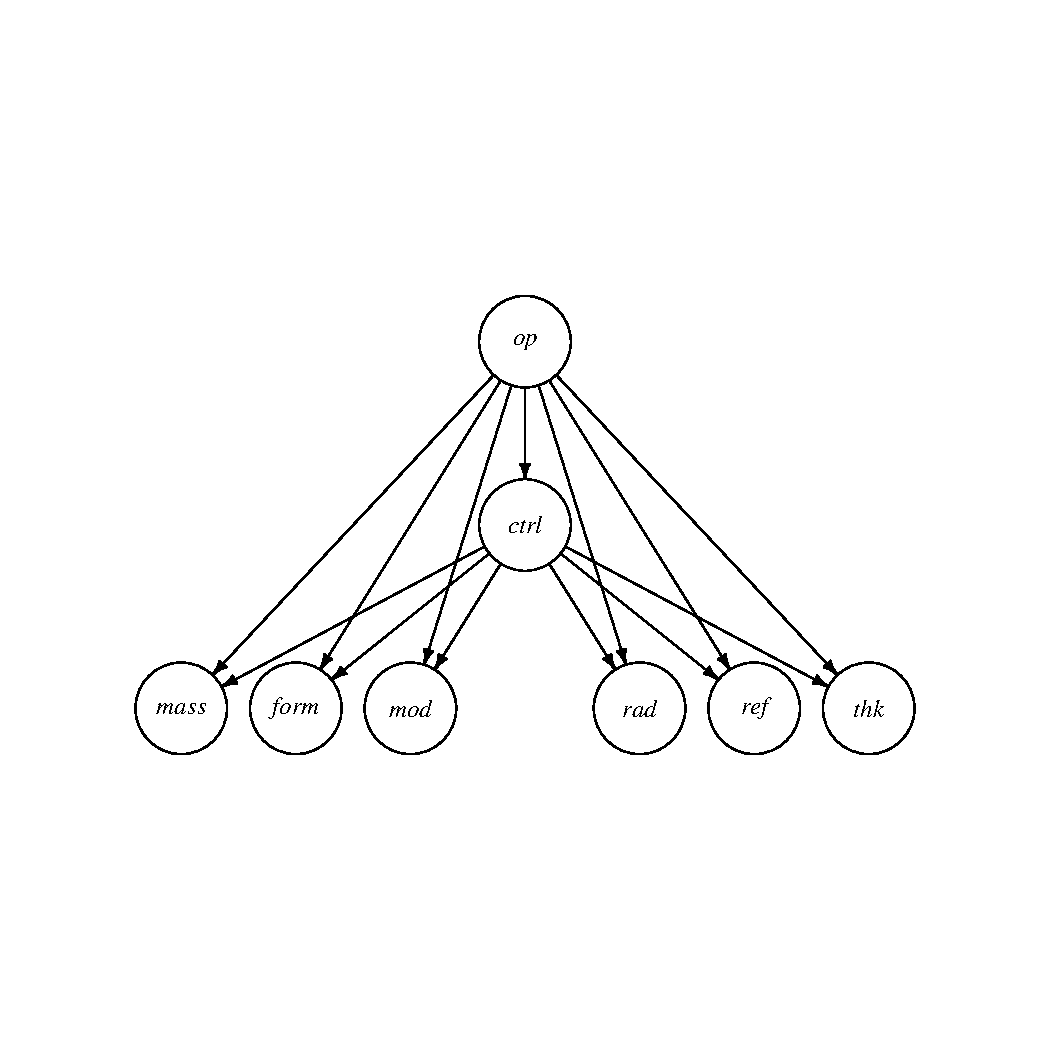
\includegraphics[trim={1cm 4.8cm 1cm 4.8cm}, width=\textwidth]{figures/bn.pdf}
  \caption{Bayesian network}
  \label{fig:bn2}
\end{figure}

The \textit{bnlearn} \cite{bnlearn} and \textit{igraph} \cite{igraph} software packages were used to build the Bayesian network and randomly sample parameters using the forward sampling algorithm (Algorithm \ref{alg:bn-fwd}).
Fissionable material operations are divided into six categories (Table \ref{table:op1}), based on safety plans and work control documents that describe each operation, as well as the criticality controls that apply to them.
Criticality controls in Building 332 consist of standardized sets of controls that are analyzed and approved for individual fissionable material operations.
Each set of controls has a single letter designation and consists of administrative limits on plutonium mass, form, moderation, and reflection (Table \ref{table:ctrl1}).
%
\begin{table}
  \caption{Fissionable material operations in Building 332}
  \label{table:op1}
  \renewcommand\arraystretch{1.5}
  \begin{center}
    \begin{tabular}{|l p{10.16cm}|}
      \hline
      operation    & description \\
      \hline
      large sample & operations with $\geq$ 65 g of plutonium \\
      machining    & operations with a drill press, grinder, lathe, mill, saw, or other cutting equipment \\
      metallurgy   & operations with a casting furnace or other heating equipment \\ 
      small sample & operations with $<$ 65 g of plutonium \\
      solution     & operations with liquids \\
      waste        & operations with radioactive waste \\
      \hline
    \end{tabular}
  \end{center}
\end{table}

\begin{table}
  \caption{Conditional probability table for fissionable material operations in Building 332}
  \label{table:op2}
  \renewcommand\arraystretch{1.5}
  \begin{center}
    \begin{tabular}{|c c c c c c|}
      \hline
      large sample & machining & metallurgy & small sample & solution & waste \\
      \hline
      0.3421       & 0.0789    & 0.1316     & 0.3158       & 0.1053   & 0.0263 \\
      \hline
    \end{tabular}
  \end{center}
\end{table}

\begin{table}
  \caption{Criticality controls in Building 332}
  \label{table:ctrl1}
  \renewcommand\arraystretch{1.5}
  \begin{center}
    \begin{tabular}{|c l l l l|}
      \hline
      condition & mass          & form               & moderation                      & reflection \\
      \hline
      A         & $\leq$ 65 g   &                    & no D$_{2}$O                     & \\
      B         & $\leq$ 220 g  &                    & H/X $\leq$ H$_{2}$O, $\leq$ 4 L & no Be/C/D$_{2}$O, $\leq$ 2 in \\
      C         & $\leq$ 1200 g &                    & $\leq$ 2.5 L                    & none \\
      D         & $\leq$ 2500 g &                    & $\leq$ 1 L                      & $\leq$ 2 L, $\leq$ 0.25 in \\
      E         & $\leq$ 2500 g &                    & none                            & $\leq$ 0.25 in \\
      M         & $\leq$ 4000 g & $\leq$ 500 g fines & $\leq$ 1 in, $\leq$ 4 L         & $\leq$ 0.3 in \\
      P         & $\leq$ 300 g  &                    & no liquids                      & $\leq$ 3.5 kg Be/C \\
      \hline
    \end{tabular}
  \end{center}
\end{table}

Most fissionable material operations have two to five sets of criticality controls.
However, only one set of criticality controls can be active at each workstation.
For example, a fissile material handler can use \textit{Condition A} at one workstation, and then switch to \textit{Condition E} if the operation requires them to move $>$ 65 grams of plutonium into the workstation.
To facilitate this move, the handler is required to ensure that the more restrictive moderator and reflector limits of \textit{Condition E} are met prior to switching from \textit{Condition A}.
The conditional probability table for each set of criticality controls (\textit{ctrl}), shown in Table \ref{table:ctrl2}, is derived from walkthrough forms, which nuclear engineers use to document active criticality controls at each workstation in the facility.

The parameters that affect nuclear criticality in Building 332 are shown in Table \ref{table:param}.
These parameters link fissionable material operations (Table \ref{table:op1}) and criticality controls (Table \ref{table:ctrl2}) to the bottom-tier Bayesian network parameters, shown in Figure \ref{fig:bn2}.
Spherical geometry and surrogate materials (Table \ref{table:param}) were selected to conservatively bound the physics of a process criticality accident.
Spherical geometry is used because a sphere has the lowest surface area-to-volume ratio of any object, which reduces neutron leakage and therefore increases $k_{eff}$ \cite{knief}.
Water is used instead of organic and inorganic liquids because it provides superior moderation and reflection, which also increases $k_{eff}$ \cite{knief}.
Polyethylene is similarly used instead of rubber, filter paper, foam, thermocouple insulation, and plastic.
Magnesium oxide (MgO) is included in Table \ref{table:param} because it is commonly used in crucibles.
Sepiolite is included because it is used to downblend plutonium oxide and absorb liquids in waste.
Other materials, such as aluminum, beryllium, depleted uranium ($^{238}$U), graphite (C), and 304 stainless steel are included because they are used in experiments or are integral to gloveboxes and process equipment.
%
\begin{table}
  \caption{Conditional probability table for criticality controls in Building 332}
  \label{table:ctrl2}
  \renewcommand\arraystretch{1.5}
  \begin{center}
    \begin{tabular}{|c l l l l l l|}
      \hline
      condition & large sample & machining & metallurgy & small sample & solution & waste \\
      \hline
      A         & 0.5714       & 0.1538    & 0.6154     & 0.9375       & 1        & 0.5 \\
      B         & 0.0286       & 0         & 0.0769     & 0.0625       & 0        & 0 \\
      C         & 0.0286       & 0         & 0          & 0            & 0        & 0 \\
      D         & 0.1714       & 0         & 0          & 0            & 0        & 0 \\
      E         & 0.0857       & 0         & 0.3077     & 0            & 0        & 0 \\
      M         & 0.1143       & 0.8462    & 0          & 0            & 0        & 0 \\
      P         & 0            & 0         & 0          & 0            & 0        & 0.5 \\
      \hline
    \end{tabular}
  \end{center}
\end{table}

\begin{table}
  \caption{Parameters that affect nuclear criticality in Building 332}
  \label{table:param}
  \renewcommand\arraystretch{1.5}
  \begin{center}
    \begin{tabular}{|l l|}
      \hline
      parameter                          & description \\
      \hline
      \textit{mass}                      & grams of plutonium (95\% $^{239}$Pu, 5\% $^{240}$Pu by weight) \\
      \textit{form}                      & plutonium in the form of alpha-phase metal or oxide (PuO$_{2}$) \\
      moderator (\textit{mod})           & MgO, CH$_{2}$, sepiolite, H$_{2}$O, or none \\
      radius (\textit{rad})              & radius of sphere (in or cm) \\
      reflector (\textit{ref})           & Al, Be, $^{238}$U, C, Pb, MgO, CH$_{2}$, \gls{ss304}, H$_{2}$O, or none \\
      reflector thickness (\textit{thk}) & reflector thickness (in or cm) \\
      \textit{shape}                     & sphere \\
      volume (\textit{vol})              & volume of sphere (cm$^{3}$) \\
      concentration (\textit{conc})      & concentration of plutonium in solution (g/cm$^{3}$) \\
      \hline
    \end{tabular}
  \end{center}
\end{table}

\section{Fitting Probability Distributions}

The probability tables for operations (\textit{op}), controls (\textit{ctrl}), \textit{form}, \textit{moderator}, and \textit{reflector} were populated directly from unclassified computer records and waste parcel cards.
The probability tables for \textit{mass}, \textit{radius}, and \textit{reflector thickness}, however, are based on truncated probability distributions (\ref{eq:gamma}-\ref{eq:weibull}) that were fit to incomplete data using the maximum likelihood estimation method \cite{d'agostino}.
Truncated gamma and normal distributions were selected because they are commonly used distributions that fit the data reasonably well (Table \ref{table:test}).
Truncated log-normal and Weibull distributions were selected because they are heavy right-tailed distributions, which increases the probability of generating random samples that result in a criticality accident.
The probability density functions of these distributions are shown in \ref{eq:gamma}-\ref{eq:weibull} \cite{devore}.
%
\begin{equation}
  \label{eq:gamma}
    \mbox{gamma distribution} \quad f(x; \alpha, \beta) = \frac{\beta^{\alpha}x^{\alpha - 1}e^{-\beta x}}{\Gamma(\alpha)} \quad x, \alpha, \beta > 0
\end{equation}

\begin{equation}
  \label{eq:normal}
  \mbox{normal distribution} \quad f(x; \mu, \sigma^{2}) = \frac{1}{\sqrt{2 \pi \sigma^{2}}} e^{\frac{(x - \mu)^{2}}{2 \sigma^{2}}}
\end{equation}

\begin{equation}
  \label{eq:log-normal}
  \mbox{log-normal distribution} \quad f(x; \mu, \sigma) = \frac{1}{\sqrt{2 \pi} \sigma x} e^{\frac{(\ln x - \mu)^{2}}{2 \sigma^{2}}}
\end{equation}

\begin{equation}
  \label{eq:weibull}
  \mbox{Weibull distribution} \quad f(x; \lambda, k) =
  \begin{cases}
    \frac{k}{\lambda} (\frac{x}{\lambda})^{k - 1} e^{-(\frac{x}{\lambda})^{k}} & x \geq 0 \\
    0 & x < 0
  \end{cases}
\end{equation}
\\
\noindent The maximum likelihood estimators are derived from the likelihood function, shown in \ref{eq:mle1}, where $X_{1}, ..., X_{n}$ are independent and indentically distributed random variables from a population with a probability density function $f(x | \theta_{1}, ..., \theta_{k}$.
%
\begin{equation}
  \label{eq:mle1}
  L(\theta | x) = L(\theta_{1}, ..., \theta_{k} | x_{1}, ..., x_{n}) = \prod_{i = 1}^{n} f(x_{i} | \theta_{1}, ..., \theta_{k})
\end{equation}

\noindent 

Once the probability distributions were fit to the data, they were trucated by selecting a conservatively large upper limit for each variable, removing values beyond the limits, and then normalizing the remaining values so that each row in the conditional probability table sums to one.
Kolmogorov-Smirnov \cite{massey}, Cram\'{e}r-von Mises, \cite{cramer}, and Anderson-Darling \cite{anderson} tests were also performed to determine the goodness of fit for each probability distribution.
The general formulas for these test statistics are shown in \ref{eq:ks}-\ref{eq:ad} \cite{anderson,cramer,massey}, where $F_{n}$ is the empirical distribution function and $F_{0}$ is the fitted cumulative distribution function.
The test statistics were calculated using the \textit{fitdistrplus} \cite{fitdistrplus} software package and compared to the critical values in R.B. D'Agostino and M.A. Stephens \cite{d'agostino}.
%
\begin{equation}
  \label{eq:ks}
  \mbox{Kolmogorov-Smirnov test statistic} \quad D = \sup_{x} | F_{n}(x) - F_{0}(x) |
\end{equation}
\vspace{+0.4cm}
\begin{equation}
  \label{eq:cvm}
  \mbox{Cram\'{e}r-von Mises test statistic} \quad W_{n}^{2} = n \int_{-\infty}^{\infty} (F_{n}(x) - F_{0}(x))^2 dF_{0}(x)
\end{equation}

\begin{equation}
  \label{eq:ad}
  \mbox{Anderson-Darling test statistic} \quad A_{n}^{2} = n \int_{-\infty}^{\infty} \frac{(F_{n}(x) - F_{0}(x))^2}{F_{0}(x)(1 - F_{0}(x))}
\end{equation}
\vspace{+0.4cm}
An example set of truncated gamma distributions and quantile-quantile (Q-Q) plots for the 65-gram \textit{Condition A} mass limit are shown in Figures \ref{fig:gamma} and \ref{fig:qq}.
Histograms of Kolmogorov-Smirnov \cite{massey}, Cram\'{e}r-von Mises, \cite{cramer}, and Anderson-Darling \cite{anderson} test statistics are shown in Figure \ref{fig:hist} and Table \ref{table:test}.
The critical values of these test statistics (Table \ref{table:test}) correspond to a significance level of $\alpha = 0.05$ with $n = 500$ samples \cite{d'agostino}.
%
\begin{figure}
  \centering
  \includegraphics[width=\textwidth]{figures/gamma.png}
  \caption{Truncated gamma distributions for 65-gram mass limit}
  \label{fig:gamma}
  \vspace{+1.1cm}
  \includegraphics[width=\textwidth]{figures/gamma-qq.png}
  \caption{Q-Q plots of truncated gamma distributions for 65-gram mass limit}
  \label{fig:qq}
\end{figure}

\begin{figure}[H]
  \centering
  \includegraphics[width=\textwidth]{figures/hist.png}
  \caption{Histograms of test statistics}
  \label{fig:hist}
\end{figure}

\begin{table}
  \caption{Test statistics}
  \label{table:test}
  \renewcommand\arraystretch{1.5}
  \begin{center}
    \begin{tabular}{|l|c c|c c|c c|}
      \multicolumn{1}{c}{} & \multicolumn{2}{c}{KS test statistic} & \multicolumn{2}{c}{CVM test statistic} & \multicolumn{2}{c}{AD test statistic} \\
      \hline
      distribution         & mean  & range                      & mean  & range                       & mean  & range \\
      \hline
      gamma                & 0.105 & 0.052-0.305                & 0.626 & 0.056-1.339                 & 3.704 & 0.333-7.909 \\
      normal               & 0.083 & 0.039-0.278                & 0.411 & 0.038-0.883                 & 2.810 & 0.301-5.787 \\
      log-normal           & 0.148 & 0.089-0.313                & 1.663 & 0.041-2.796                 & 9.870 & 0.271-16.348 \\
      Weibull              & 0.081 & 0.029-0.307                & 0.305 & 0.020-0.802                 & 2.126 & 0.158-5.581 \\
      \hline
      critical value       & \multicolumn{2}{c|}{0.061}         & \multicolumn{2}{c|}{0.220}          & \multicolumn{2}{c|}{0.751-0.795} \\
      \hline
    \end{tabular}
  \end{center}
\end{table}

The results shown in Table \ref{table:test} indicate that the test statistics for the truncated gamma, normal, and Weibull distributions fit the data slightly better than the truncated log-normal distributions---although this is by no means a definitive assessment of each fit.
The purpose of calculating these test statistics is to document the goodness of fit, which is commonly used in conjunction with graphical checks of Q-Q plots (Figure \ref{fig:qq}) to validate risk models in the nuclear industry.

\section{Generating Random Samples}

The Bayesian network forward sampling algorithm (\ref{alg:bn-fwd}) is used to generate random samples, which are passed to the neural network metamodel.
